\documentclass{article}
\usepackage{enumitem}
\usepackage[T1]{fontenc}
\usepackage[utf8]{inputenc}
\usepackage[portuguese]{babel}
\usepackage[vmargin=3cm]{geometry}
\usepackage{tikzpagenodes}
\usepackage{lipsum}
\usepackage{xcolor}
\usepackage{cancel}
\usepackage{amsmath}
\usepackage{mathrsfs}
\usepackage{amssymb}
\usepackage{background}
\usepackage{titlesec}
\usepackage[nodisplayskipstretch]{setspace}
\usepackage{hyphenat}
\usepackage[normalem]{ulem}
\usepackage{minted}
\usepackage{subcaption}
\usepackage{tikz}
\hyphenation{mate-mática recu-perar}
\titlespacing{\section}{0pc}{-0.25em}{0pc}
\titlespacing{\subsection}{0pc}{0em}{0pc}
\titlespacing{\subsubsection}{0pc}{0.33em}{0pc}
\titlespacing{\paragraph}{0em}{0.25em}{0.5em}
\setlength{\parindent}{2em}
\setlength{\parskip}{1em}
\linespread{1}

\renewcommand{\baselinestretch}{1.0}

\renewcommand\bf[1]{\textbf{#1}}
\renewcommand\it[1]{\textit{#1}}

\newcommand\ov[1]{\overline{#1}}
\newcommand{\vect}[1]{\mathbf{#1}}
\newcommand{\bb}[1]{\mathbb{#1}}
\newcommand{\vn}{\varnothing}
\newcommand\stk[2][black]{\setbox0=\hbox{$#2$}%
\rlap{\raisebox{.45\ht0}{\textcolor{#1}{\rule{\wd0}{1pt}}}}#2}

\makeatletter
\global\let\tikz@ensure@dollar@catcode=\relax
\makeatother

\makeatletter
\def\mcolor#1#{\@mcolor{#1}}
\def\@mcolor#1#2#3{%
  \protect\leavevmode
  \begingroup
    \color#1{#2}#3%
  \endgroup
}
\makeatother
\definecolor{notepadrule}{RGB}{217,244,244}

\backgroundsetup{
contents={%
  \begin{tikzpicture}
    \foreach \fila in {0,...,52}
    {
      \draw [line width=1pt,color=notepadrule]
      (current page.west|-0,-\fila*12pt) -- ++(\paperwidth,0);
    }
    \draw[overlay,red!70!black,line width=1pt]
      ([xshift=-1pt]current page text area.west|-current page.north) --
      ([xshift=-1pt]current page text area.west|-current page.south);
  \end{tikzpicture}%
},
scale=1,
angle=0,
opacity=1
}

\begin{document}

\setlength{\abovedisplayskip}{12pt}
\setlength{\belowdisplayskip}{12pt}
\setlength{\abovedisplayshortskip}{0pt}
\setlength{\belowdisplayshortskip}{0pt}
% \setlength{\baselineskip}{12pt}
\setlength{\jot}{3pt}

\section{Exercício - Teorema da Inversão}
Considere $X$ uma variável aleatória com PDF $f_X$ e CDF $F_X(x)$. Considere ainda $U \sim
\mathscr{U}([0,1))$. Defina $g:\bb{R} \rightarrow \bb{R}$ tal que $g(u) = F^{-1}(u)$ ($F$ é suposta
inversível). Qual a PDF de $Y=g(U)$?

\bf{Resolução:} Para um dado $y \in ([a,b]), \; \exists! \; u \in \bb{R} / g(u_i) = y$ e $u =
F_X(y)$
\begin{align*}
    f_Y(y) &= \sum_i \frac{f_U(u_i)}{|g'(u_i)|} \\
    f_Y(y) &= \sum_i \frac{f_U(F_X(y))}{|g'(u_i)|} \text{, não nulo em } \forall \; y \in ([a,b]) \\
    F_X(g(u)) &= u, \; g \text{ é inversa de } F_X \\
    F_X'(g(u)) \cdot g'(u) &= 1 \\
    g'(u) &= \frac{1}{F_X'(g(u))} \\
    f_U(y) &=
        \begin{cases}
            0, y \notin ([a,b]), \\[0.5em]
            \frac{f_U(F_X(y))}{|F_X'(g(F_X(y)))|^{-1}}, y \in ([a,b]) \\
        \end{cases} \\
        g(F_X(y)) &= y, \text{ pois } g = F_X^{-1} \\
        \text{Finalmente:} \\
    f_Y(y) &=
        \begin{cases}
            0, y \notin ([a,b]), \\[0.5em]
            \frac{\mcolor{red}{f_U(F_X(y))}}{|F_X'(y)|^{-1}}, y \in ([a,b]) \\
        \end{cases} \\
    &\mcolor{red}{f_U(F_X(y))} \text{ é cte. e vale 1} \\
    f_Y(y) &=
        \begin{cases}
            0, y \notin ([a,b]), \\[0.5em]
            |F_X'(y)|, y \in ([a,b]) \\
        \end{cases} \\
        & \text{A derivada da CDF é a PDF e o valor abs. é indiferente, obtemos:} \\
    f_Y(y) &=
        \begin{cases}
            0, y \notin ([a,b]), \\[0.5em]
            f_X(y), y \in ([a,b]) \\
        \end{cases} \\
        & ([a,b]) \text{ é a imagem da função g considerando o domínio [0,1)} \\
        & f_Y(y) = f_X(y), \text{ se considerarmos y válido (na imagem de g)}
\end{align*}

\newpage
\section{Aplicação do Teorema da Inversão}
Considere uma variável aleatória $X$ com PDF $f_X(x)$ "linear entre -2 e 4"

\subsection*{a)} Implemente um gerador pseudoaleatório que gere realizações dessa v.a.
\begin{align*}
    f_X(x) &=
        \begin{cases}
            0, x \leq 2, \\
            \frac{x+2}{18}, -2 < x \leq 4 \\
            0, x > 4, \\
        \end{cases}
    &F_X(x) =
        \begin{cases}
            0, x \leq 2, \\
            \int_{-2}^x \frac{\lambda + 2}{18} d\lambda = \frac{x^2+4x+4}{36}, -2 < x \leq 4 \\
            1, x > 4, \\
        \end{cases}
\end{align*}

\begin{align*}
    g(u) = F_X^{-1}(x) =
        \begin{cases}
            -2, \text{ se } u = 0 \\
            4, \text{ se } u = 1 \\
            6 \sqrt{u} - 2, \text{ se } 0 < u < 1
        \end{cases}
\end{align*}

\subsection*{b)}

\begin{minted}[breaklines, linenos]{matlab}
clear all; close all; clc;

% x values to test theoretical model
xt = linspace(-2.5, 4.5, 1e4);
f_Xteo = pdf_g(xt);
% Test using our (pseudo) random number generator
N = 1e6;
[x, x_values, f_X] = exampleRandGen(N);

% Plots
plot(x_values, f_X);
hold on;
plot(xt, f_Xteo);
set(findall(gcf,'type','text'), 'FontSize', 30, 'fontWeight', 'bold');
ylabel('f_X');
xlabel('x');
set(gcf, 'Color', 'w');
set(gca, 'FontName', 'Inconsolata Nerd Font', 'FontSize', 20, 'FontWeight', 'bold');
set(gca, 'XMinorTick', 'on', 'YMinorTick', 'on')
set(gca, 'XGrid', 'on', 'YGrid', 'on');
set(gca, 'XMinorGrid', 'on', 'YMinorGrid', 'on');
legend({['Empirical N=' int2str(N)], 'Theoretical'}, 'Location', 'northwest');

%% Using function from exercise B to gen random values
function [x, x_values, f_X] = exampleRandGen(N)
    if ~exist('N', 'var') || isempty(N)
        N = 100;
    end
    u = rand(N, 1);
    x = g(u);
    [f_X, x_values] = pdf_empirical_evaluation(x, min(round(N/10), 1000));
end

function x = g(u)
    x = zeros(size(u));
    x(u == 0) = -2;
    x(u == 1) = 4;
    x(u ~= 0 & u ~= 1) = -2 +6 * sqrt(u(u ~= 0 & u ~= 1));
end

function [p] = pdf_g(x)
    p = zeros(size(x));
    k = find(x > -2 & x < 4);
    p(k) = (x(k)+2)/18;
end

function [epdf, bins_centers] = pdf_empirical_evaluation(x, nbins)
    if ~exist('nbins', 'var') || isempty(nbins)
        nbins = 1000;
    end
    [h, bins_centers] = hist(x, nbins);
    bin_width = (bins_centers(2:end) - bins_centers(1:end-1));
    bin_width = mean(bin_width);
    epdf = (h/length(x))/bin_width;
end
\end{minted}

\begin{figure}[H]
    \centering
    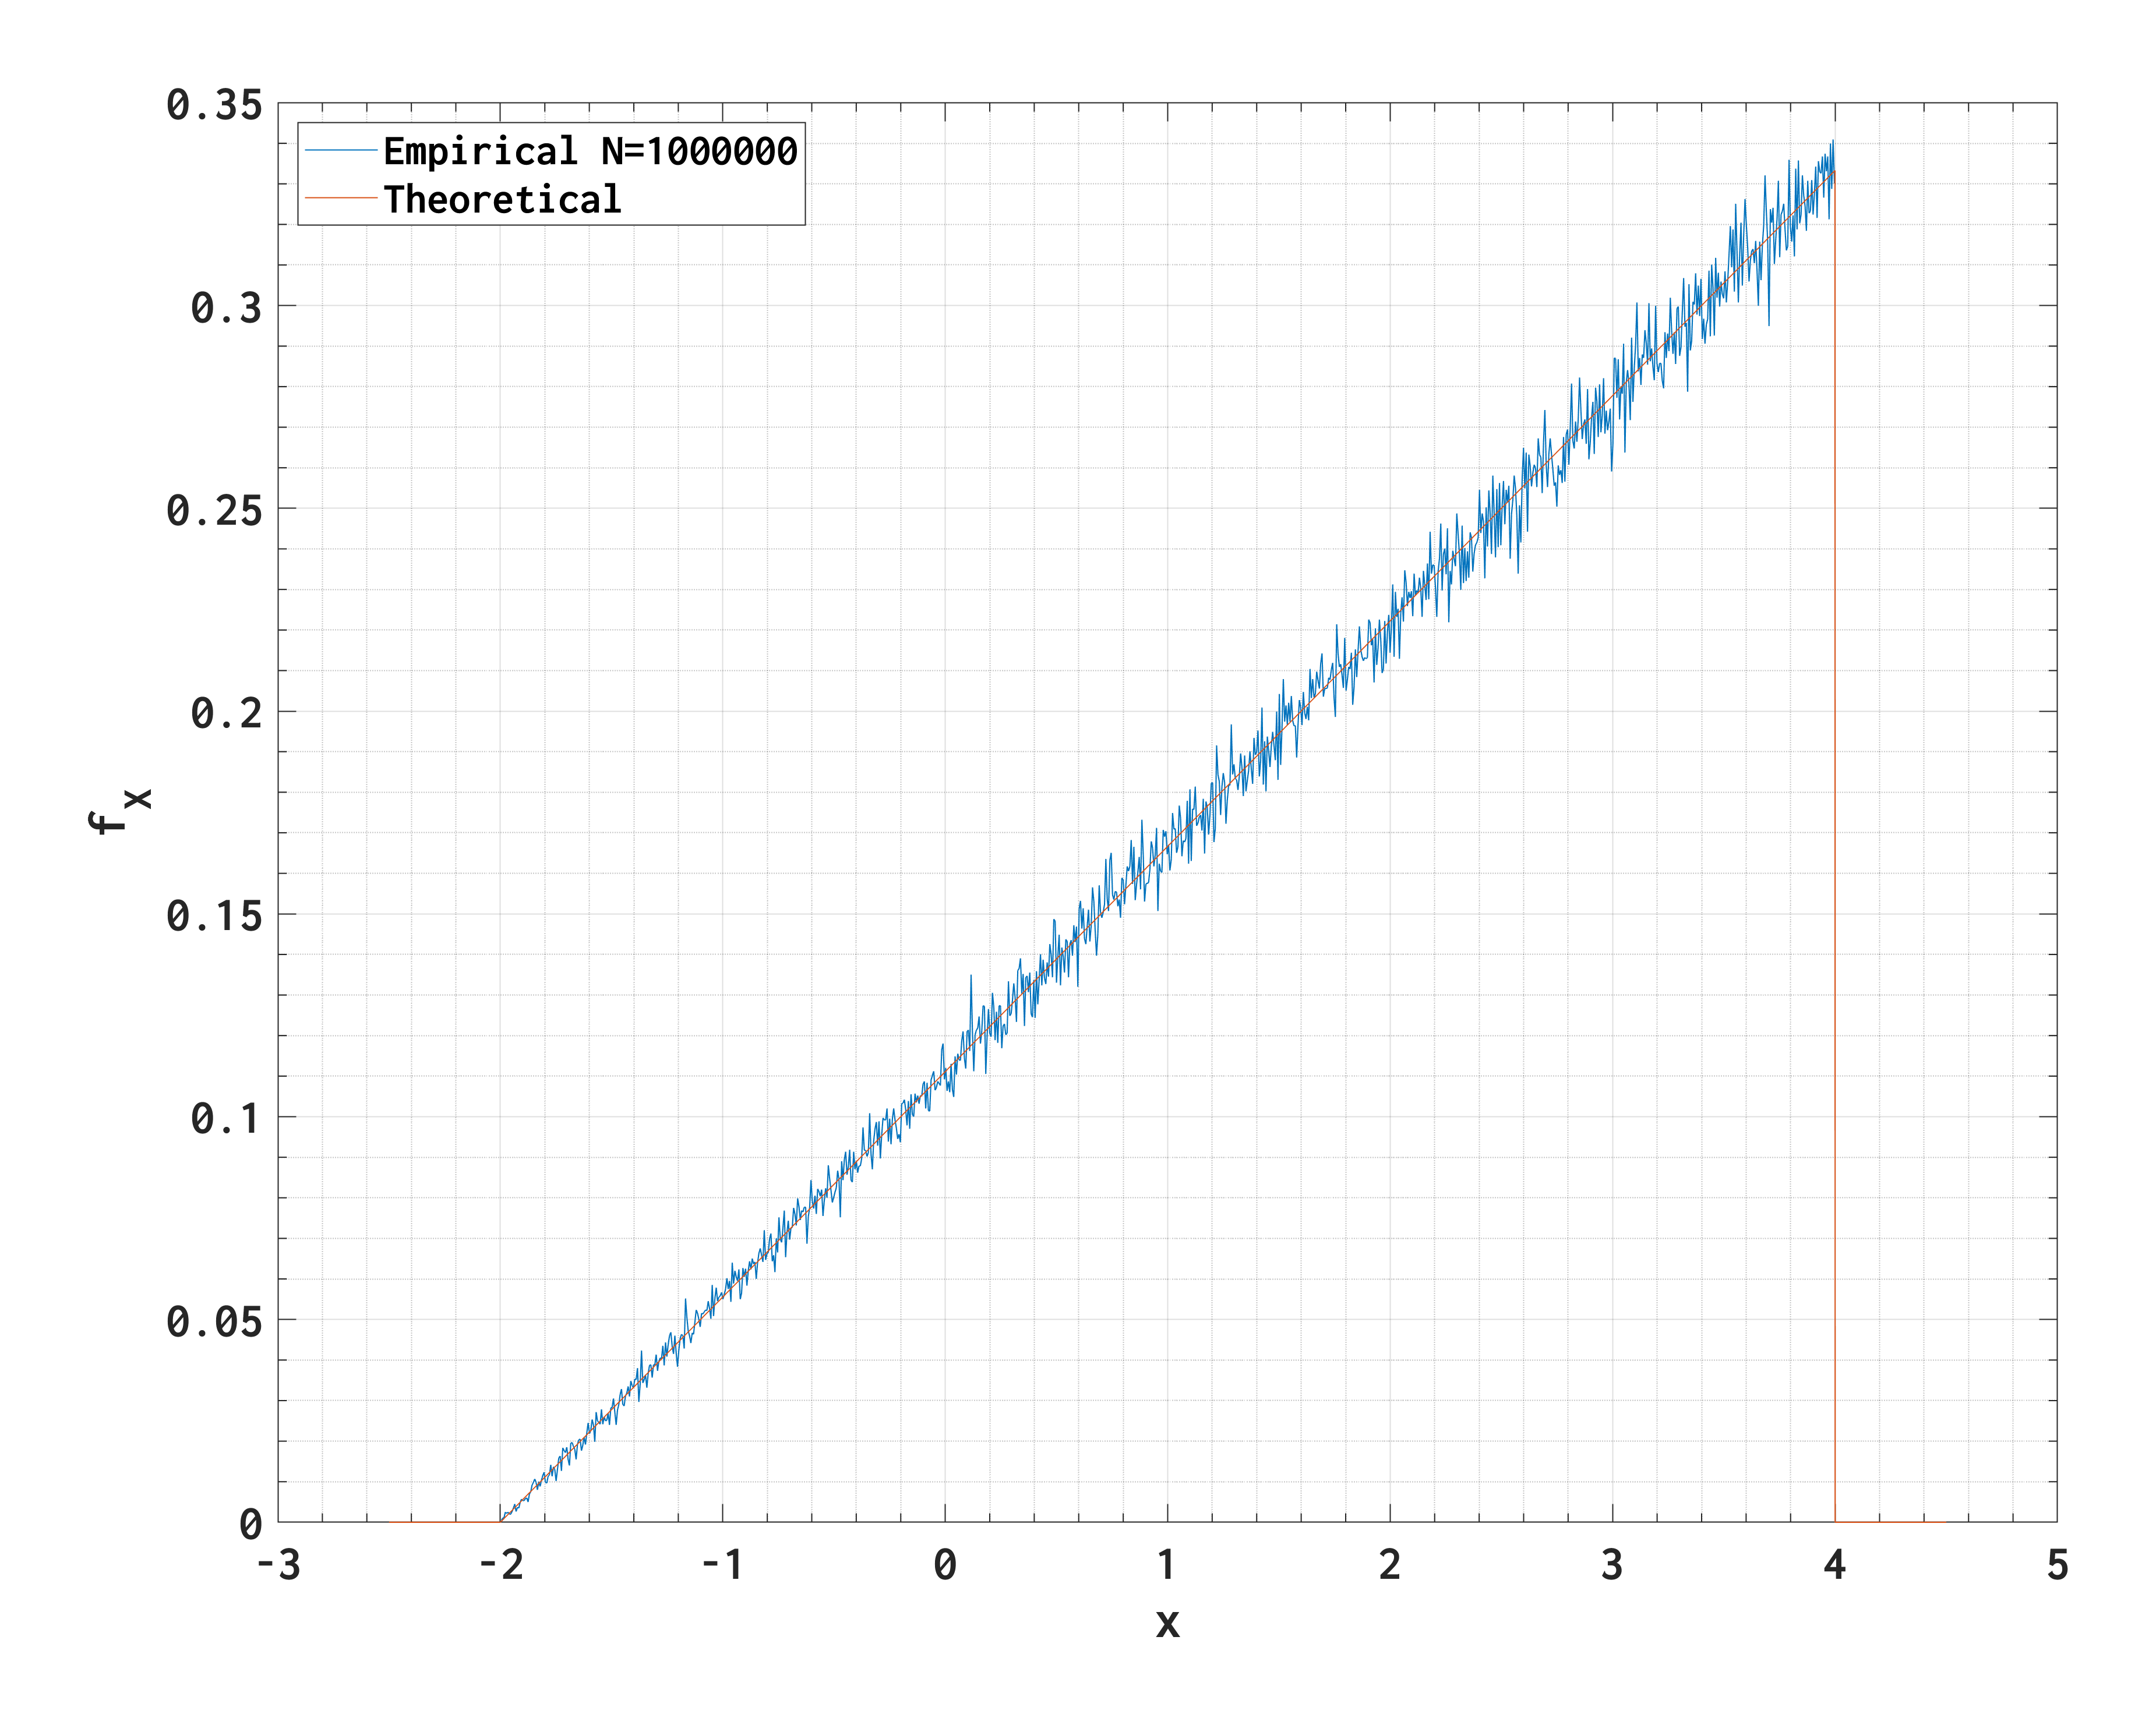
\includegraphics[scale=0.35]{figures/b_pdf-plot.png}
    \caption{PDF para Modelo Teórico e Empírico do item b}
    \label{fig:pdf_B}
\end{figure}


\end{document}
